\section{Other segmentation methods}
Besides the above methods, there are also lots of other image segmentation methods. The watershed method, which is a kind of region growing method, is very useful for merging cell dividing. The clustering based methods, such as K-Means and mean shift, can be used to efficiently label an image.
\subsection{Watershed method}
Watershed method\cite{vincent1991watersheds} is a region-based segmentation approach for grayscale image segmentation. It simulates the rain falling and dam building process, which is demoed in Fig\ref{fig:imgseg-watershed}. For image segmentation, this method divides an image into many catchment basins, which are the regions of an image, where the water will not flow into other region. The most successful application of watershed method is to segment two overlap cells. Usually we need to perform distance transfrom on the cell image.

An efficient way to compute such regions is to start raining from all the local minimas and to label the flooded area with the same label to its local minima's. The flooding process can be implemented using a priority queue of pixels and breadth-first search. See Alg\ref{alg:imgseg-watershed} for Vincent and Soile's water flooding method\cite{vincent1991watersheds}.

The main problem for the proposed watershed algorithm (Alg\ref{alg:imgseg-watershed}) is that there are usually lots of local minimas, which will segment an image into many pieces. It is necessary to filter these local minimas by filtering on some features. Another way to solve this problem is to manually define a seed for each regions, which can be used as an interative segmentation method.


\begin{figure}[htbp]
\centering
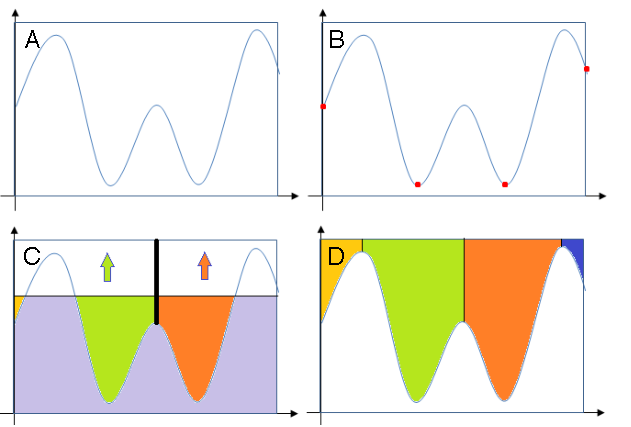
\includegraphics[width=1.0\textwidth]{images/imgseg_watershed}
\caption[The process of watershed method on 1D image]{The process of watershed method on 1D image. A. Original 1D signals. B. The local minimas detected. C. The bottom up flooding process. D. Final segmentation result.}
\label{fig:imgseg-watershed}
\end{figure}

\begin{algorithm}[H]
\SetAlgoLined
Generate a list of all pixels in the image in height order\;
Pixels belonging to the minimum are labeled with different identifier and placed into a FIFO queue\;
\ForEach{pixel in the queue}{
	Removed the top pixel from the queue and put its unvisited neighbors into the queue\;
	\If{The top pixel's neighboring have only one kind of labeled identifier}{
		Label it with the same identifier\;
	}
	\Else{
		Label it with watershed line\;
	}
}
\caption{Vincent and Soile's water flooding method}
\label{alg:imgseg-watershed}
\end{algorithm}

\section{Open-source librarys}
There are lots implementation codes for the above methods, 
\subsection{ITK}
\subsection{OpenCV}
\subsection{My work}
